\documentclass{article}
\usepackage{amsthm}
\usepackage{amsmath}

%%%%%%%%%%%%%%%% Tikz and pgf %%%%%%%%%%%%%%%%%%%%%5
\usepackage{tikz}
%\usepackage{pgfmath}
\usetikzlibrary{positioning, arrows,automata}
\usetikzlibrary{shapes}

%%%%%%%%%%%%%%%%%%%%%%%%%%%%%%%%%%%%%%%%%%%%%%%%%%%%%





\newtheorem{theorem}{Theorem}[section]
\title{How to make money using Number theory?}
\author{Dofus M Bofus}
\begin{document}
\maketitle

\section{Introduction}

For a complex number $s$, we consider the series.

\begin{equation}
  \zeta(s) = \sum_{n=1}^\infty \frac{1}{n^s}
  \label{eq-riemann-zeta}
\end{equation}

\begin{theorem}
  Consider the analytic continuation of the \emph{Riemann zeta function}
  defined in Equation~\ref{eq-riemann-zeta}. All the non-trivial roots
  of it lie on the $\mathrm{Re}(s)=\frac{1}{2}$ line.
\end{theorem}



\section{Plotting graphs}

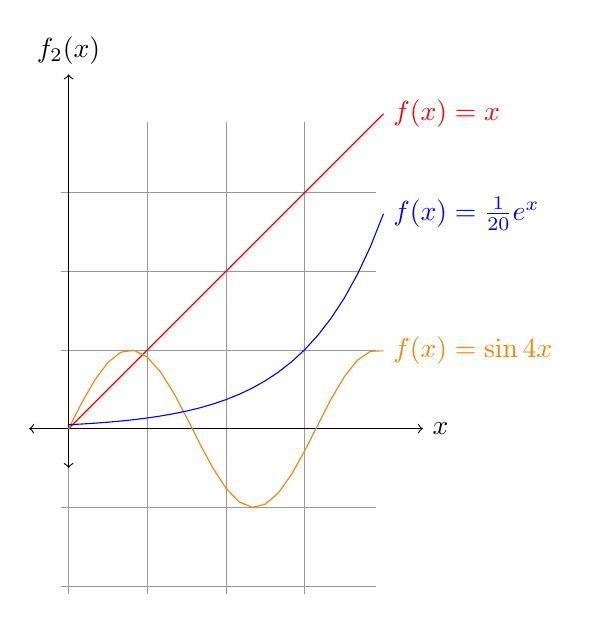
\begin{tikzpicture}[domain=0:4]
  \draw[very thin, color=black!40] (-0.1,-2.1) grid (3.9,3.9);
  \draw[<->] (-0.5,0) -- (4.5,0) node [right] {$x$};
  \draw[<->] (0,-0.5) -- (0,4.5)  node [above] {$f_2(x)$};
  \draw[color=red] plot (\x,\x) node [right] {$f(x) = x$};
  \draw[color=orange] plot (\x,{sin(2*\x r)}) node [right] {$f(x) = \sin {4}x$};
  \draw[color=blue] plot (\x,{0.05*exp(\x)}) node [right] {$f(x) = \frac{1}{20}e^x$};
\end{tikzpicture}


\end{document}
